\chapter[Interleaf Pages]{Interleaf Pages (Páginas Intercaladas)}

Páginas intercaladas são páginas que são inseridas entre partes de um documento. Tradicionalmente, essas páginas são completamente em branco. O \LaTeX, no entanto, as define por padrão com o estilo de página atual. O \KOMAScript\ fornece várias extensões para essa funcionalidade.

Páginas intercaladas são encontradas principalmente em livros. Como os capítulos de livros geralmente começam na página direita (frente) de uma página dupla, uma página esquerda (verso) vazia deve ser inserida se o capítulo anterior terminar em uma página frente. Por esse motivo, as páginas intercaladas realmente só existem para impressão frente e verso.
\begin{center}
    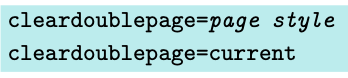
\includegraphics[width=0.5\linewidth]{imagens/imagem15.png}
\end{center}
Com esta opção, você pode definir o estilo de página das páginas intercaladas criadas pelos comandos \char`\\\texttt{clear\-dou\-ble\-pa\-ge} \char`\\\texttt{clear\-dou\-ble\-odd\-pa\-ge}  ou \char`\\\texttt{clear\-dou\-ble\-e\-ven\-pa\-ge} para avançar para a página desejada. Você pode usar qualquer estilo de página definido anteriormente (consulte a seção 3.12 da página 80 e capítulo 5 da página 255). Além disso, \texttt{clear\-dou\-ble\-pa\-ge=cur\-rent} também é possível. Este caso corresponde ao padrão anterior ao \KOMAScript~2.98c e cria uma página intercalada sem alterar o estilo da página. A partir do \KOMAScript~3.00, o padrão segue a recomendação da maioria dos tipógrafos e cria páginas intercaladas com o estilo de página vazio, a menos que você altere a compatibilidade para versões anteriores do \KOMAScript\ (consulte a opção versão, seção 3.2, página 55).

\textbf{Exemplo}: Suponha que você queira páginas intercaladas que estejam vazias, exceto pela paginação, para que elas sejam criadas com \texttt{plain}. Você pode conseguir isso, por exemplo, com:

\begin{verbatim}
        \KOMAoptions{cleardoublepage=plain}
\end{verbatim}

Você pode encontrar mais informações sobre o estilo de página simples (\textbf{plain page style}) na seção 3.12, página 81.

O kernel do \LaTeX\ fornece o comando \verb|\clear\-page|, que garante que todos os \textbf{floats} pendentes sejam exibidos e então inicie uma nova página. Há também o comando \char`\\\texttt{clear\-dou\-ble\-pa\-ge}, que funciona como \verb|\clear\-page|, mas que inicia uma nova página à direita na impressão frente e verso (veja a opção de layout frente e verso na seção 2.4, página 40). Uma página vazia à esquerda no estilo de página atual é exibida, se necessário.

\begin{figure}[hb]
    \centering
    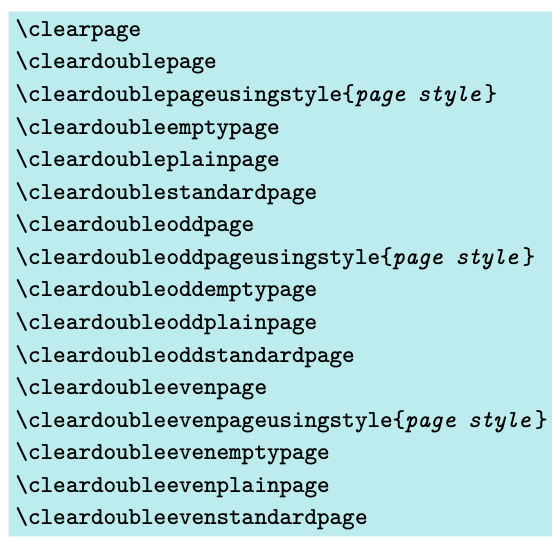
\includegraphics[width=0.75\linewidth]{imagens/imagem16.png}
    %\caption{Enter Caption}
    \label{fig:img16}
\end{figure}


    
